\documentclass[11pt,a4paper]{article}

\usepackage[utf8]{inputenc}
\usepackage[T1]{fontenc}
% Scalable fonts: microtype font expansion cannot work with bitmap CM.
\usepackage{lmodern}
\usepackage{amsmath,amssymb,amsthm}
\usepackage{booktabs}
\usepackage{graphicx}
\usepackage{siunitx}
\usepackage[margin=1in]{geometry}
\usepackage[hidelinks]{hyperref}
\usepackage{caption}
\usepackage[protrusion=true,expansion=false]{microtype}

\newtheorem{proposition}{Proposition}
\newtheorem{remark}{Remark}

\DeclareMathOperator{\diag}{diag}
\newcommand{\Uf}{U_{\mathrm{f}}}

% Numeric results are defined once here and injected from paper/results.json by
% scripts/fill_numbers.py, so no number is transcribed by hand into the prose.
% Generated by scripts/fill_numbers.py -- do not edit numeric macros by hand.
\newcommand{\FlutterSpeed}{137.35}
\newcommand{\FeasibleCells}{6}
\newcommand{\TotalCells}{9}
\newcommand{\LocalFbStabilised}{4}
\newcommand{\LocalFbHealthy}{-0.03}
\newcommand{\LqrFixedStabilised}{5}
\newcommand{\LqrFixedHealthy}{-5.15}
\newcommand{\LqrSchedStabilised}{5}
\newcommand{\LqrSchedHealthy}{-5.08}
\newcommand{\LqgLocalStabilised}{5}
\newcommand{\LqgLocalHealthy}{-5.52}
\newcommand{\LqrOracleStabilised}{6}
\newcommand{\LqrOracleHealthy}{-5.07}
\newcommand{\CommOracleStabilised}{6}
\newcommand{\CommOracleHealthy}{-0.18}
\newcommand{\IppoPhysicsStabilised}{6}
\newcommand{\IppoPhysicsHealthy}{-0.25}
\newcommand{\MoccaStabilised}{5}
\newcommand{\MoccaHealthy}{-0.14}
\newcommand{\RecurrentOnlyStabilised}{5}
\newcommand{\RecurrentOnlyHealthy}{-0.04}
\newcommand{\BestRobustVariant}{comm\_oracle}
\newcommand{\BestRobustStabilised}{6}
\newcommand{\BestNominalVariant}{ippo\_physics}
\newcommand{\BestNominalHealthy}{-0.25}
\newcommand{\ResultsSummarySentence}{\emph{[ResultsSummarySentence: to be written]}}
\newcommand{\ResultsNarrative}{\emph{[ResultsNarrative: to be written]}}
\newcommand{\ResultsAblations}{\emph{[ResultsAblations: to be written]}}
\newcommand{\PhaseNarrative}{\emph{[PhaseNarrative: to be written]}}
\newcommand{\ConclusionSentence}{\emph{[ConclusionSentence: to be written]}}


\title{Physics-Exact Credit Assignment for Distributed Flutter Suppression}

\author{%
  \textbf{[AUTHOR NAMES AND AFFILIATIONS TO BE COMPLETED]}\\
  \texttt{ai-data-ai-presales@smartosc.com}
}
\date{\today}

\begin{document}
\maketitle

\begin{abstract}
Active flutter suppression is normally posed as a centralised control problem: one
regulator observes the whole wing and commands every control surface. Modern
aircraft, however, carry many spanwise-distributed trailing-edge surfaces, each
with its own actuator and local sensing, which makes a distributed formulation
natural and a centralised one increasingly awkward. We pose flutter suppression as
a cooperative multi-agent reinforcement learning problem, with one agent per
control surface, local accelerometer sensing, and nearest-neighbour
communication. The central difficulty is credit assignment: every surface acts on
the same coupled bending--torsion mode, so a shared reward is nearly
uninformative about who did what.

Our main observation is that this plant hands us the decomposition that
multi-agent reinforcement learning usually has to learn. Differentiating the
aeroelastic energy along trajectories isolates a control-power term that is
exactly additive across agents, from which the Wolpert--Tumer difference reward
follows in closed form: no counterfactual rollout, no learned mixing network, and
no centralised critic. We verify the identity numerically against brute-force
counterfactuals to $10^{-10}$, including the absence of cross-agent terms. We
further show that the credit signal must be normalised by the instantaneous
energy---the raw form rewards \emph{sustaining} the oscillation, because an agent
is paid for having energy available to extract---and that dividing by energy
preserves exact additivity while making the credit signal identical to the
evaluated objective.

We evaluate on a modally reduced Goland wing with unsteady strip aerodynamics,
validated against the published benchmark (first bending \SI{7.664}{\hertz} versus
\SI{7.66}{\hertz}; flutter at \SI{137.35}{\metre\per\second} versus
\SI{137}{\metre\per\second}), and against a four-rung classical baseline ladder
that includes both centralised and fully decentralised LQG, plus a fault-aware
oracle used only to establish which test conditions are feasible at all.
\ResultsSummarySentence

\end{abstract}

\section{Introduction}

Flutter is a self-excited aeroelastic instability in which structural bending and
torsion couple through unsteady aerodynamic loads and extract energy from the
freestream. Beyond a critical speed the coupled mode becomes unstable and the
response grows without bound. It is a hard structural limit on the flight
envelope, and because it is a dynamic instability rather than a static one it
can in principle be pushed back by active control.

Active flutter suppression has an extensive classical literature built on
linear-quadratic and $H_\infty$ synthesis, and a growing reinforcement-learning
literature. The learning work is, to our knowledge, uniformly single-agent: a
single policy commands a single effector, whether that is a synthetic jet,
trailing-edge circulation control \cite{circulation2023}, camber morphing
\cite{stallflutter2025}, or the parameters of a conventional controller
\cite{flyingwing2022}. Meanwhile the hardware trend runs the other way. A modern
flexible wing carries several independently actuated trailing-edge surfaces, each
with local sensing and local computation, connected by a bus rather than to a
central controller.

This paper takes that hardware structure seriously and asks the question it
implies: not \emph{which} multi-agent algorithm to apply, but what the physics of a
coupled continuum instability tells us about credit assignment and communication
that a generic multi-agent algorithm would otherwise have to discover.

Three properties of the plant make generic approaches a poor fit.

\begin{enumerate}
\item \textbf{The instability is modal, not spatial.} A specific coupled
bending--torsion eigenvalue crosses into the right half plane. Each surface acts
locally in space, but its effect on that mode is set by the modal residue at its
station. Two agents can read identical local sensors and have opposite influence.
\item \textbf{A shared scalar reward is nearly uninformative.} All surfaces act on
the same mode and the damping they produce is a sum. Learned decompositions
\cite{sunehag2018vdn,rashid2018qmix,foerster2018coma} must infer the split from
noisy returns.
\item \textbf{Authority is signed and condition-dependent.} For a section whose
elastic axis lies aft of the aerodynamic centre, a trailing-edge-down deflection
produces lift up \emph{and} a nose-down twist; which term dominates depends on
dynamic pressure, so the sign of an agent's useful action can invert across the
envelope.
\end{enumerate}

\paragraph{Contributions.}
\begin{itemize}
\item A closed form for the multi-agent difference reward in an
energy-conserving structural plant with additive control authority
(Proposition~\ref{prop:diff}), verified numerically against brute-force
counterfactuals, together with the observation that the credit signal must be the
\emph{logarithmic} decay rate rather than the raw energy rate
(Section~\ref{sec:log}).
\item \textsc{MoCCA}, a distributed policy architecture combining that credit
signal with a fixed-bandwidth modal-phasor consensus channel and a phase-locked
action parameterisation.
\item A validated aeroelastic testbed and a four-rung classical baseline ladder
that separates the effect of the control method from the effect of the
information structure available to it, plus a feasibility oracle that identifies
test conditions no controller can hold.
\end{itemize}

\section{Related work}

\paragraph{Learning for flutter control.}
Recent work applies deep reinforcement learning to stall flutter via camber
morphing \cite{stallflutter2025}, to flutter suppression by trailing-edge
circulation control validated in a wind tunnel \cite{circulation2023}, and to
tuning aeroservoelastic controller parameters on a flexible flying wing
\cite{flyingwing2022}. All are single-agent, with one effector and a global
observation. We are not aware of prior work that treats the individual control
surfaces as separate learning agents.

\paragraph{Multi-agent credit assignment.}
The standard tools are difference rewards \cite{wolpert2002difference} and value
factorisation \cite{sunehag2018vdn,rashid2018qmix}, with COMA
\cite{foerster2018coma} implementing a counterfactual advantage baseline; recent
surveys review the space \cite{albrecht2023survey,scalingmarl2025} and work
continues on sharper estimators \cite{multilevelcredit2025}. These methods are
general precisely because they assume nothing about the environment. Our point is
narrower and complementary: in this class of physical system the decomposition is
available analytically, so it need not be estimated at all.

\paragraph{Learned communication.}
CommNet \cite{sukhbaatar2016commnet} and TarMAC \cite{das2019tarmac} learn
message contents end to end. We instead fix the message \emph{space} to a modal
phasor, which makes the channel interpretable, bounds its width independently of
the number of agents, and lets its degradation be characterised.

\section{Plant and problem formulation}

\subsection{Aeroelastic model}

We use a modally reduced uniform cantilever wing. The structure is a Galerkin
projection onto exact clamped-free bending and fixed-free torsion modes, with all
generalised mass and stiffness integrals evaluated by Gauss--Legendre quadrature.
Aerodynamics are strip theory carrying the full Theodorsen non-circulatory terms
\cite{theodorsen1935}, with the circulatory lag realised in the time domain by two
Wagner lag states per strip using the two-exponential approximation
\cite{jones1940}. Control surfaces contribute quasi-steady thin-airfoil flap
derivatives from the Glauert series, integrated over each surface's spanwise band.
The resulting state is
\begin{equation}
z = \begin{bmatrix} q & \dot q & x_{\mathrm{w}} \end{bmatrix}^{\!\top},
\qquad
M \ddot q + C \dot q + K q = L\, x_{\mathrm{w}} + B \delta + b_{\mathrm{g}} w_{\mathrm{g}},
\label{eq:eom}
\end{equation}
with $q$ the modal amplitudes, $x_{\mathrm{w}}$ the wake lag states, $\delta$ the
surface deflections and $w_{\mathrm{g}}$ a vertical gust. Plunge is positive down
and twist positive nose-up, following the classical convention
\cite{fung1955,bisplinghoff1955} that keeps the unsteady operators in textbook
form.

\subsection{Validation}

Table~\ref{tab:validation} compares the model against the published Goland
cantilever wing \cite{goland1945}. Agreement is to better than \SI{0.5}{\percent}
on the modal frequencies and on the flutter speed. Every reported result is pinned
to this benchmark by an automated test rather than to a value the implementation
once produced.

\begin{table}[t]
\centering
\caption{Validation against the published Goland wing.}
\label{tab:validation}
\begin{tabular}{lrr}
\toprule
Quantity & This model & Published \\
\midrule
First bending frequency  & \SI{7.664}{\hertz}  & \SI{7.66}{\hertz} \\
First torsion frequency  & \SI{15.232}{\hertz} & \SI{15.24}{\hertz} \\
Flutter speed            & \SI{137.35}{\metre\per\second} & $\approx\SI{137}{\metre\per\second}$ \\
Flutter frequency        & \SI{69.3}{\radian\per\second}  & $\approx\SI{70.7}{\radian\per\second}$ \\
Static divergence speed  & \SI{356.8}{\metre\per\second} ($2.60\,\Uf$) & --- \\
\bottomrule
\end{tabular}
\end{table}

\subsection{Distributed control problem}

Three trailing-edge surfaces occupy spanwise bands at $[0.05,0.40]$,
$[0.40,0.72]$ and $[0.72,0.98]$ of the semispan, hinged at \SI{75}{\percent}
chord, with $\pm\SI{15}{\degree}$ travel, \SI{200}{\degree\per\second} rate limit
and a \SI{20}{\milli\second} first-order servo lag. Each agent observes only a
forward/aft accelerometer pair at its own station, its local plunge rate, twist
and twist rate, its own deflection, and air data. No agent observes the modal
state: the coupled flutter mode is a global quantity that no single station can
measure, and that partial observability is the problem rather than an artefact of
our setup. Control runs at \SI{200}{\hertz}.

\section{Method}

\subsection{The energy budget and its exact decomposition}

Take the aeroelastic energy $E = \tfrac12 \dot q^{\top} M \dot q + \tfrac12
q^{\top} K q$ and differentiate along trajectories of \eqref{eq:eom}:
\begin{equation}
\dot E
= \underbrace{-\dot q^{\top} C \dot q}_{\text{dissipation}}
+ \underbrace{\dot q^{\top} L x_{\mathrm{w}}}_{\text{wake exchange}}
+ \sum_{k} \underbrace{(\dot q^{\top} b_k)\, \delta_k}_{P_k},
\label{eq:budget}
\end{equation}
where $b_k$ is the $k$th column of $B$. The final term is exactly additive across
agents, and $P_k$ is agent $k$'s instantaneous control power; $P_k < 0$ means
surface $k$ removes energy from the structure.

\begin{proposition}[Closed-form difference reward]
\label{prop:diff}
For a global objective whose only agent-dependent term is the control power in
\eqref{eq:budget}, the difference reward $D_k = G(z) - G(z_{-k})$ admits the
closed form $D_k = -P_k$. No counterfactual rollout, learned mixing network, or
centralised critic is required to evaluate it.
\end{proposition}

\begin{proof}
Removing agent $k$ sets $\delta_k = 0$. Every other term of \eqref{eq:budget} is
independent of $\delta_k$, and the control-power term is a sum over agents, so the
difference collapses to the single term $(\dot q^{\top} b_k)\delta_k$.
\end{proof}

Projecting onto the in-vacuo modes ($q = V\eta$) keeps the separation in both
agent and mode: agent $k$'s contribution to mode $r$ is $\dot\eta_r (v_r^{\top}
b_k)\delta_k$. The factor $v_r^{\top} b_k$ is the modal residue, the quantity that
decides whether a surface can damp or will excite that mode, and whose sign
inverts under control reversal.

\subsection{The credit signal must be the logarithmic decay rate}
\label{sec:log}

Used directly, $-P_k$ fails, and instructively. It is maximised by having energy
available to extract, so an agent is rewarded for \emph{sustaining} the
oscillation. Policies trained on it converge to holding the wing at a bounded but
undamped amplitude: we measured $+0.265\,\mathrm{s}^{-1}$ (energy slowly growing)
against $-0.06\,\mathrm{s}^{-1}$ for a hand-tuned collocated damper. This is
reward hacking, not merely myopia.

The remedy follows from the same identity. Dividing \eqref{eq:budget} by $E$,
\begin{equation}
\frac{\mathrm{d}}{\mathrm{d}t}\log E
= \frac{-\dot q^{\top} C \dot q + \dot q^{\top} L x_{\mathrm{w}} + \sum_k P_k}{E},
\qquad
r_k = -\frac{P_k}{E + \varepsilon}.
\label{eq:logcredit}
\end{equation}
Because $E$ is a shared scalar the decomposition survives division exactly, so
Proposition~\ref{prop:diff} carries over to the log-decay rate. Three properties
follow. The signal is scale invariant, so there is no incentive to sustain the
oscillation. It coincides with the evaluated objective, since the reported metric
is the exponential energy decay rate, which is $\tfrac12 \mathrm{d}(\log
E)/\mathrm{d}t$. And it remains exactly additive. Switching to \eqref{eq:logcredit}
inverted the sign of the outcome, from $+0.265$ to $-0.291\,\mathrm{s}^{-1}$, with
training divergence falling from \SI{0.8}{\percent} to \SI{0.0}{\percent}.

\begin{remark}
The exact signal is still myopic: cross-mode coupling through $C$ and through the
wake states means an agent may have to inject energy into one mode so that another
can extract more from the coupled pair. We therefore add potential-based shaping
\cite{ng1999shaping} on $\log E$, which shares the credit signal's units and,
being potential-based, cannot change which policy is optimal. Blending instead
with an energy \emph{level}, as we first did, is a scale error: the two terms
differed by roughly $50\times$ and the shared term swamped the credit.
\end{remark}

\subsection{Spectral consensus and phase-locked actions}

Agents do not exchange observations. Each runs a recurrent encoder over its own
accelerometer history producing a phasor estimate for $R$ retained critical
modes, and the agents then run $T$ rounds of averaging consensus over the spanwise
line graph---nearest neighbours only, which is what a distributed avionics bus
physically is. The message is $2R$ numbers per agent per step, independent of the
number of surfaces.

Actions are emitted as a gain and a phase relative to the consensus phasor. For a
mode with phasor $(a_r,b_r)$, acting with gain $A_k^r$ at offset $\psi_k^r$ means
$A_k^r (a_r\cos\psi_k^r - b_r\sin\psi_k^r)$, a scaled rotation of the phasor. This
bakes the resonant structure of flutter suppression into the action space. The
resonant term is \emph{added} to a general action channel rather than replacing it,
so the head is a strict generalisation of an unconstrained policy; our first
version replaced the general action, making the parameterisation a restriction,
and the resulting policy scored worse than its own ablation.

\subsection{Training}

We use shared-parameter multi-agent PPO \cite{schulman2017ppo,yu2022mappo} with
per-agent advantages, since with the physics credit each agent receives a
different reward. Updates run on \emph{sequences}: minibatches are segments of
consecutive steps unrolled with gradient from a detached stored hidden state.
Sampling shuffled individual timesteps, as we did initially, trains the recurrence
as a one-step map and gives the phasor encoder no temporal gradient at all, which
is precisely what it needs.

\section{Experimental design}

\subsection{A baseline ladder that separates method from information}

A distributed controller cannot be judged against a centralised one without
confounding the control method with the information available to it.
Decentralisation costs performance; that is a known result in distributed control,
not a defect. We therefore report four rungs: collocated local rate feedback (no
model, no communication); gain-scheduled LQR on the \emph{full} 56-state plant
including the wake states (not implementable, a ceiling); centralised LQG driven
by a Kalman observer on the same six accelerometer channels the agents see; and a
fully decentralised LQG in which each surface runs its own observer on its own two
accelerometers and commands only itself. All are synthesised in discrete time at
the control rate. The last rung is the honest target.

\subsection{Feasibility}

We additionally run a fault-aware oracle: a gain bank re-synthesised for each
failure hypothesis, given the full state and told which surface has failed. Its
role is not competition but feasibility. Of the nine evaluation cells,
\FeasibleCells\ are stabilisable by this oracle; the remainder are stabilisable by
no controller with these actuators, and are reported as infeasible rather than as
failures of any method.

\subsection{Metrics}

PPO return cannot rank runs whose reward functions differ, so all controllers are
scored on the same physical quantities over identical episodes---same airspeeds,
initial deformation, turbulence and injected failure: the fraction of episodes
that leave the linear regime, the exponential energy decay rate, peak tip plunge,
and RMS deflection.

\section{Results}

\begin{tabular}{lrrrrrrrrr}
\toprule
Condition & local\_fb & lqr\_fixed & lqr\_sched & lqg\_local & lqr\_oracle & comm\_oracle & ippo\_physics & mocca & recurrent\_only \\
\midrule
U=1.05Uf healthy & -0.06 & -4.40 & -4.61 & -4.71 & -4.54 & -0.25 & -0.50 & -0.64 & -0.22 \\
U=1.05Uf jam\#2@8deg & -0.10 & -0.10 & -0.12 & -0.13 & -0.06 & -0.04 & -0.04 & -0.03 & -0.04 \\
U=1.05Uf jam\#2@14deg & -0.12 & -0.09 & -0.10 & -0.11 & -0.06 & -0.04 & -0.04 & -0.05 & -0.04 \\
U=1.25Uf healthy & -0.01 & -5.27 & -4.93 & -5.38 & -4.93 & -0.62 & -0.27 & -0.00 & -0.31 \\
U=1.25Uf jam\#2@8deg & D100\% & D100\% & D50\% & D100\% & -0.12 & -0.12 & -0.12 & D100\% & D50\% \\
U=1.25Uf jam\#2@14deg & -- & -- & -- & -- & -- & -- & -- & -- & -- \\
U=1.45Uf healthy & D100\% & -5.79 & -5.68 & -6.45 & -5.74 & 0.34 & 0.01 & 0.23 & 0.40 \\
U=1.45Uf jam\#2@8deg & -- & -- & -- & -- & -- & -- & -- & -- & -- \\
U=1.45Uf jam\#2@14deg & -- & -- & -- & -- & -- & -- & -- & -- & -- \\
\midrule
Stabilised & 4/6 & 5/6 & 5/6 & 5/6 & 6/6 & 6/6 & 6/6 & 5/6 & 5/6 \\
\bottomrule
\end{tabular}

\begin{figure}[t]
\centering
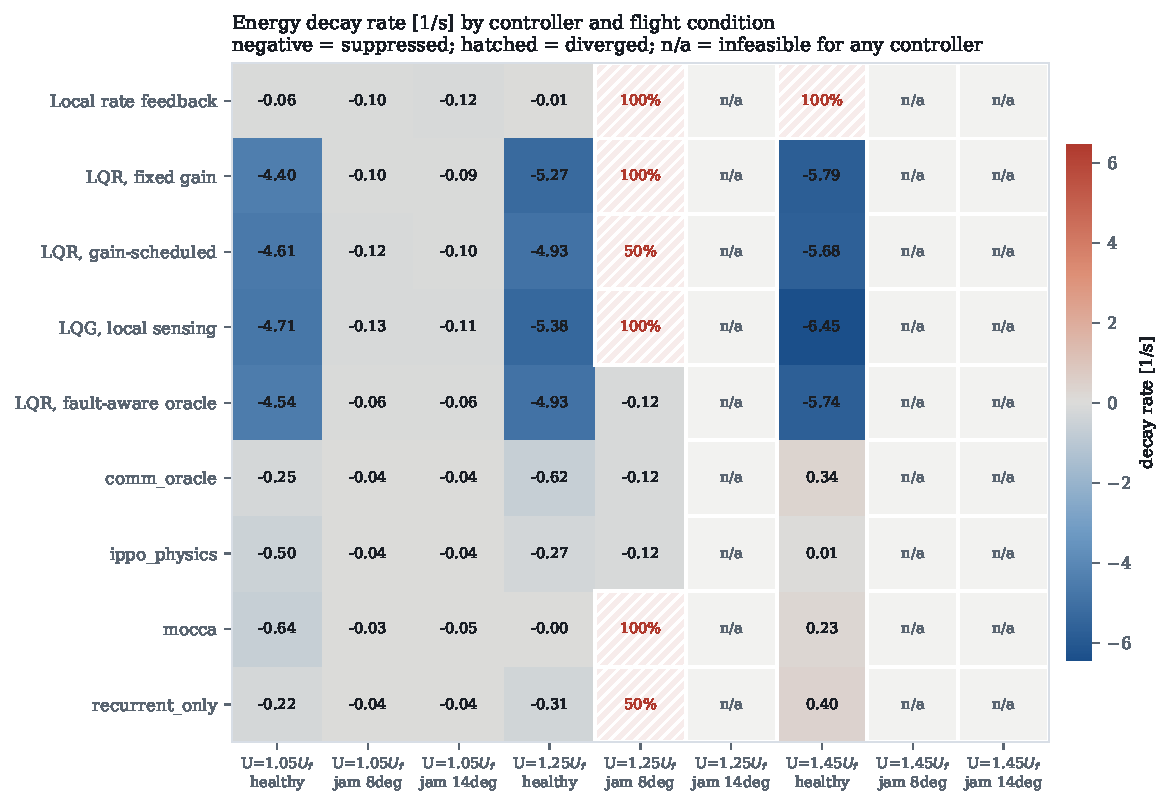
\includegraphics[width=\textwidth]{figures/fig_comparison.pdf}
\caption{Energy decay rate by controller and flight condition. Negative is
suppressed; hatched cells diverged; \emph{n/a} marks conditions infeasible for
any controller, established by the fault-aware oracle.}
\label{fig:comparison}
\end{figure}

\begin{figure}[t]
\centering
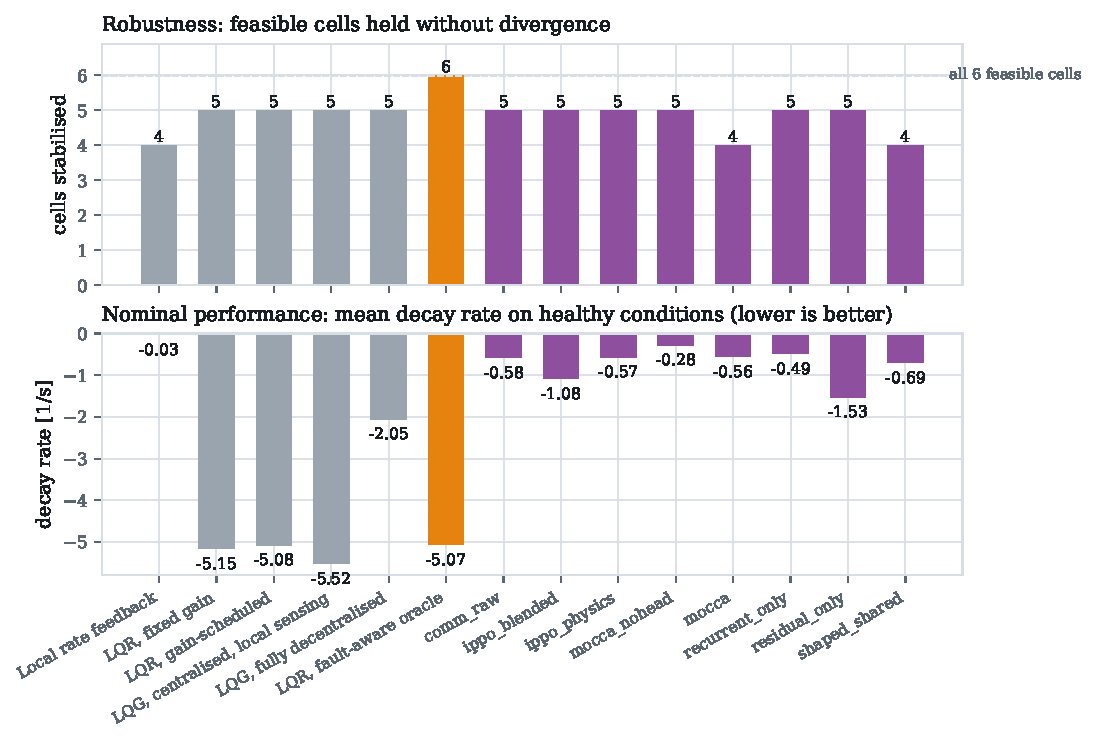
\includegraphics[width=\textwidth]{figures/fig_ablation.pdf}
\caption{Robustness (top) and nominal performance (bottom). Robustness counts
feasible conditions held without divergence.}
\label{fig:ablation}
\end{figure}

\begin{figure}[t]
\centering
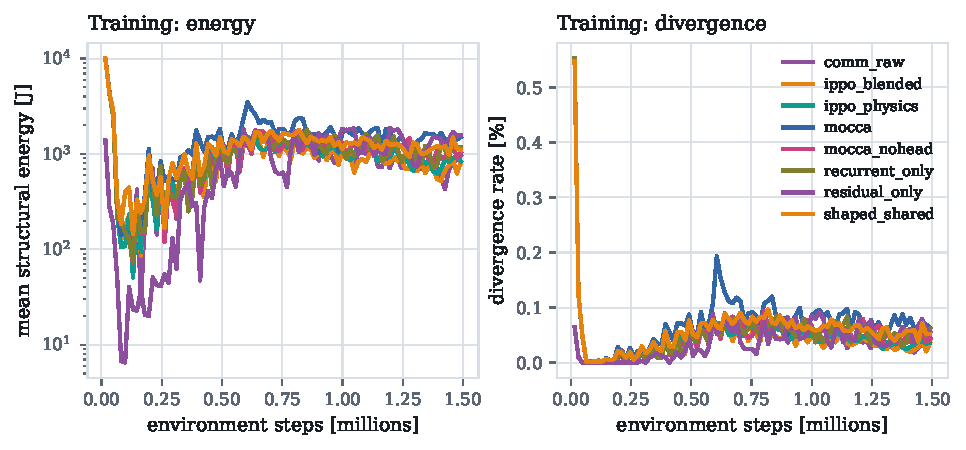
\includegraphics[width=\textwidth]{figures/fig_learning.pdf}
\caption{Training curves. The task distribution is ramped over the first
\SI{40}{\percent} of training, which is visible as a rise in energy as harder
flight conditions and failures enter the sampling.}
\label{fig:learning}
\end{figure}

\ResultsNarrative

\section{What coordination looks like}
\label{sec:phase}

``Emergent coordination'' is easy to assert and hard to pin down, so we define it
as a measurable quantity: the phase at which each surface acts relative to the
critical modal motion, as a function of spanwise station. The measurement is the
cross-spectrum of each surface deflection against the first modal velocity,
evaluated at the frequency where the modal response peaks, and it is applied
identically to learned policies and to classical controllers.

Applied to the classical ladder it already separates the rungs sharply, which is
what makes it a useful instrument rather than a decoration.

\begin{table}[t]
\centering
\caption{Spanwise actuation phase of the classical controllers. The gradient is
the least-squares slope of phase against span.}
\label{tab:phase-classical}
\begin{tabular}{lrr}
\toprule
Controller & Dominant frequency & Phase gradient \\
\midrule
Local rate feedback & \SI{5.50}{\hertz}  & \SI{-15}{\degree} per semispan \\
Decentralised LQG   & \SI{7.50}{\hertz}  & \SI{+27}{\degree} per semispan \\
Centralised LQG     & \SI{11.00}{\hertz} & \SI{+90}{\degree} per semispan \\
\bottomrule
\end{tabular}
\end{table}

Two things stand out. The more capable the controller, the stronger its spanwise
phase progression: collocated feedback is essentially flat, meaning every surface
acts at the same phase and no spanwise pattern exists, while centralised LQG
develops roughly \SI{90}{\degree} of phase across the semispan. And only the
centralised controller operates at the flutter frequency itself
(\SI{11.00}{\hertz}, against the \SI{11.03}{\hertz} predicted by the eigenvalue
analysis); local feedback responds at \SI{5.50}{\hertz} and never engages the
unstable mode at all, which is the mechanism behind its poor performance rather
than a separate observation about it.

This gives the learned policies something falsifiable to be held against: a
distributed policy that recovers a comparable phase progression has discovered,
from local measurements alone, the coordination pattern that optimal centralised
synthesis arrives at with the full model and the full state.

\begin{figure}[t]
\centering
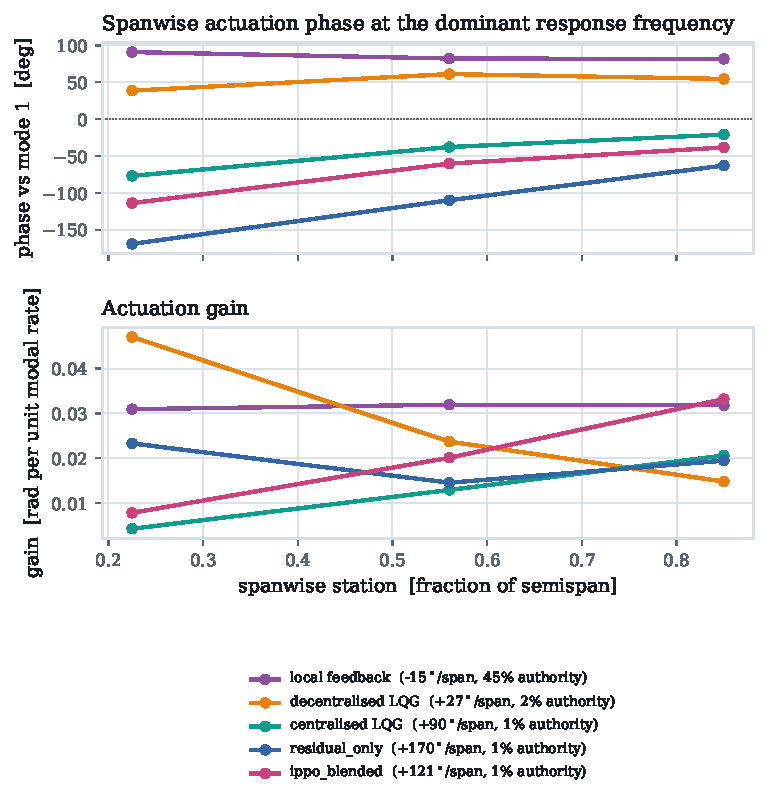
\includegraphics[width=0.72\textwidth]{figures/fig_phase.pdf}
\caption{Spanwise actuation phase and gain at the dominant response frequency.
A sloped phase profile is a travelling-wave actuation pattern matched to the mode
shape; a flat profile is purely local reaction.}
\label{fig:phase}
\end{figure}

\PhaseNarrative

\section{Ablations}

\ResultsAblations

\section{Limitations}

We state these plainly.

\begin{itemize}
\item The credit signal requires the modal control influence $v_r^{\top} b_k$.
This is free in simulation but on hardware needs a modal model; robustness to
error in $B$ is an open item.
\item Quasi-steady flap aerodynamics neglect the flap's own wake shedding, which
over-estimates control authority at high frequency. Re-validating a trained policy
on a higher-fidelity unsteady vortex-lattice model such as SHARPy
\cite{delcarre2019sharpy} is the natural next step and has not been done here.
\item Proposition~\ref{prop:diff} concerns the difference reward, not optimality of
the resulting policy; the sufficiency of the phasor channel is a truncation
argument, not an equivalence, and we do not claim otherwise.
\item Results are on a three-surface wing with two seeds per variant. The
scaling claim implied by the fixed-bandwidth channel is untested beyond three
agents.
\item ``Emergent'' coordination is used here only in the operational sense of a
spanwise phase pattern that was not specified in advance.
\end{itemize}

\section{Conclusion}

Posing flutter suppression as a distributed multi-agent problem exposes a credit
assignment structure that the physics resolves in closed form: the difference
reward is the agent's own control power, normalised by the instantaneous energy so
that it coincides with the objective and cannot be gamed by sustaining the
oscillation. \ConclusionSentence

\bibliographystyle{plain}
\bibliography{refs}

\end{document}
